
\documentclass[12pt]{article}
\usepackage{graphicx}
\usepackage{hyperref}
\usepackage{amsmath}


\begin{document}

\begin{center}
\textbf{ MAT 442: HMW 6}\\
\textbf{\ ERICAGYEMANG (Spring 2019)}\\
\end{center}

\begin{enumerate} 
\item Problem 16:

(a) \[x_{t+1}=r+x_t+x^2_t\] 
To find the equilibrium points, we set 
\begin{align*}
&f(x)=r+x+x^2=x\\
&\Rightarrow x^2+r=0
\end{align*}
Using the quadratic formula we obtain
\begin{align*}
x&=\frac{0\pm 2\sqrt{-r}}{2}= \pm \sqrt{-r}=\boxed{ \sqrt{-r} \hspace{0.3cm}\mbox{or}\hspace{0.2cm} -\sqrt{-r}.}
\end{align*}

Since the derivative of 
\[f(x)=r+x+x^2\]
is
\[\boxed{f'(x)=2x+1},\]
it follows that when $x=\sqrt{-r}$ , $f'(\sqrt{-r})=1+2\sqrt{-r}>1$ so that $x=\sqrt{-r}$ is unstable.But for $x=-\sqrt{-r}$ , $f'(-\sqrt{-r})=1-2-\sqrt{-r}$ so that for $-1<r<0$, we have $\left|f'(-\sqrt{-r})\right|<1$ thus equilibrium $x=-\sqrt{-r}$ is LAS.Therefore the bifurcation diagram has the form given below.

\begin{figure} [ht!]
 \centering
 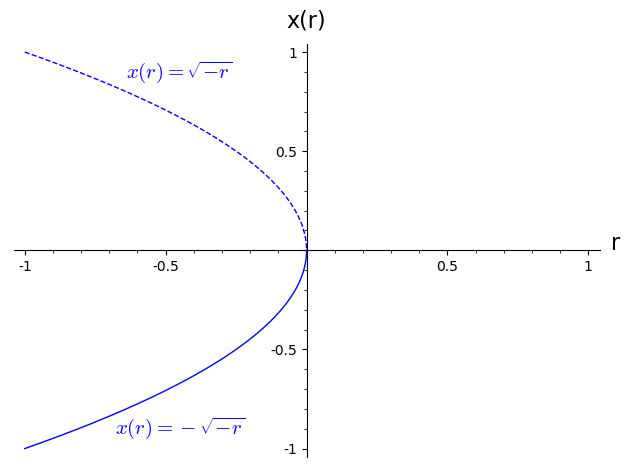
\includegraphics[height=4in]{/Users/ERICAGYEMANG/Desktop/Biomath/Figures/tmpsix.jpg} 
        \caption[Figure 2.4: r>1]{The dashed curve in the graph represents unstability and the solid curve represents stability.}
 \label{fig::model}
\end{figure}


\cleardoublepage
(b) \[x_{t+1}=(r+1)x_t-x_t^3\] 
To find the equilibrium points, we set 
\begin{align*}
&f(x)=(r+1)x-x^3=x\\
&\Rightarrow -x+x(r+1)-x^3=0\\
&\Rightarrow x(r-x^3)=0
\end{align*}
Using the quadratic formula we obtain
\begin{align*}
x&=\frac{0\pm 2\sqrt{r}}{2}= \pm \sqrt{r}=\boxed{ x=0\hspace{0.2cm} \mbox{or} \hspace{0.2cm} \sqrt{r} \hspace{0.3cm}\mbox{or}\hspace{0.2cm} -\sqrt{r}}.
\end{align*}

Since the derivative of 
\[f(x)=(r+1)x-x^3\]
is
\[\boxed{f'(x)=r+1-3x^2},\]
it follows that when $x=0$ , $f'(0)=r+1$ and set $-1<r+1<1$ as usual so that $-2<r<0$ is unstable.

Howerver, for $x=\sqrt{r}$ , $f'(\sqrt{r})=r+1-3r$ we have
\[-1<r+1-3r<1 \Leftrightarrow -2<-2r<0 \Leftrightarrow \boxed{ 0<r<1}\] which is stable
and for $x=-\sqrt{r}$ , $f'(-\sqrt{r})=r+1+3r$ we get
\[-1<r+1+3r<1 \Leftrightarrow -2<4r<0 \Leftrightarrow \boxed{ -1/2<r<0}\] which is also stable.

Therefore the bifurcation diagram has the form given below.

\begin{figure} [ht!]
 \centering
 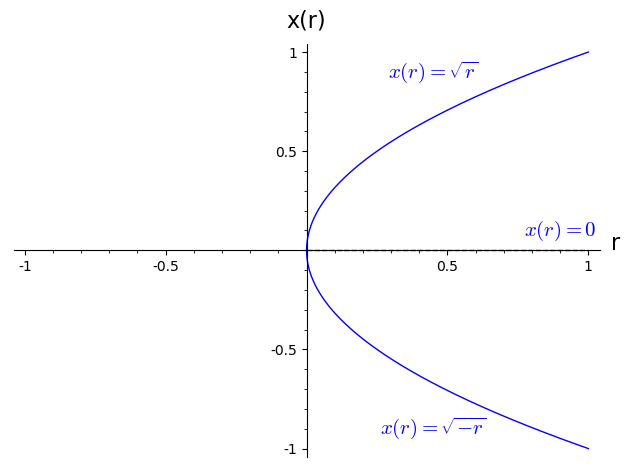
\includegraphics[height=4in]{/Users/ERICAGYEMANG/Desktop/Biomath/Figures/tmpsixx.jpg} 
        \caption[Figure 2.4: r>1]{The dashed line in the graph represents unstability and the solid curve represents stability.}
 \label{fig::model}
\end{figure}

\cleardoublepage
(c) \[x_{t+1}=(r+1)x_t+x_t^2\] 
To find the equilibrium points, we set 
\begin{align*}
&f(x)=(r+1)x+x^2=x\\
&\Rightarrow -x+x(r+1)+x^2=0\\
&\Rightarrow rx+x^2=0
\end{align*}
Using the factor method we obtain
\begin{align*}
&\Rightarrow x(r+x)=0\\
&\Rightarrow \boxed{x=0\hspace{0.1cm} \mbox{or} \hspace{0.1cm} x=-r}.
\end{align*}

Since the derivative of 
\[f(x)=(r+1)x+x^2\]
is
\[\boxed{f'(x)=r+1+2x},\]
it follows that when $x=0$ , $f'(0)=r+1$ and set $-1<f'(0)<1$ as usual to get \boxed{-2<r<0} so that $x=0$ is unstable.But for $x=-r$, $f'(-r)=r+1+2(-r)$ we set $-1<f'(0)<1$ as usual to get
\[-1<-r+1<1\Leftrightarrow -2<-r<0 \Leftrightarrow \boxed{0<r<2}\]
thus r is stable.Therefore the bifurcation diagram has the form given below.

\begin{figure} [ht!]
 \centering
 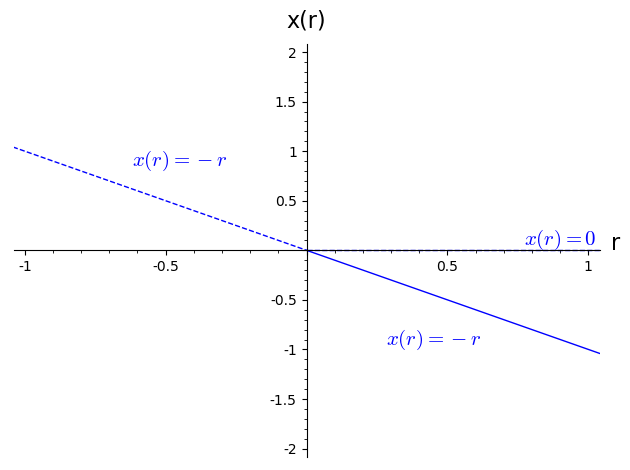
\includegraphics[height=4in]{/Users/ERICAGYEMANG/Desktop/Biomath/Figures/tmpsixxx.jpg} 
        \caption[Figure 2.4: r>1]{The dashed line in the graph represents unstability and the solid lines represents stability.}
 \label{fig::model}
\end{figure}

\cleardoublepage


\item Problem 17:

 \[x_{t+1}=r-x_t-x^2_t\] 
To find the equilibrium points, we set 
\begin{align*}
&f(x)=r-x-x^2=x\\
&\Rightarrow -r+2x+x^2=0
\end{align*}
Using the quadratic formula we obtain
\begin{align*}
x&=\frac{-2\pm \sqrt{4r+4}}{2}= -1\pm \sqrt{r+1}=\boxed{ \sqrt{r+1}-1 \hspace{0.3cm}\mbox{or}\hspace{0.2cm} -\sqrt{r+1}-1.}
\end{align*}

Since the derivative of 
\[f(x)=r-x-x^2\]
is
\[\boxed{f'(x)=-1-2x}.\]
Now to check for the stability we have $1+r>0\Leftrightarrow r>-1$.Then
\[f'(-1+\sqrt{r+1})=-1-2(-1+\sqrt{1+r})=1-2\sqrt{1+r},\]
 and as always we set 
 \[-1<1-\sqrt{1+r}<1\Leftrightarrow 1>\sqrt{1+r}>0 \Leftrightarrow 0<1+r<1 \Leftrightarrow \boxed{-1<r<0}\]
 Hence r is stable.
 For
  \[f'(-1-\sqrt{1+r})=-1-2(-1-\sqrt{1+r})=1+2\sqrt{1+r}>1\]  is unstable.\\
 
 
 For 2-cycle,I used $mathematica$ command \[\mbox{solve}[f[f[x]]==x,x]\] to give us the solutions 
 \[-\sqrt{r},\sqrt{r},-1-\sqrt{1+r},-1+\sqrt{1+r}.\]
 Since $f'(y)=-1-2y$
 we compute
 \[f'(-\sqrt{r})= -1+2(\sqrt{r})\hspace{0.1cm} \mbox{and}\hspace{0.1cm} f'(\sqrt{r})= -1-2\sqrt{r} .\]
 Now to check the stability of the 2-cycles, we have
 \[f'(-\sqrt{r})f'(\sqrt{r})=(-1+2\sqrt{r})(-1-2\sqrt{r})=1-4\sqrt{r}\]
 thus
 \[-1<1-4r<1 \Leftrightarrow -2<-4r<0 \Leftrightarrow 0<4r<2 \Leftrightarrow \boxed{0<r<1/2}\]
 Therefore 2-cycles is LAS.The bifurcation diagram has the form given below.

\cleardoublepage

\begin{figure} [ht!]
 \centering
 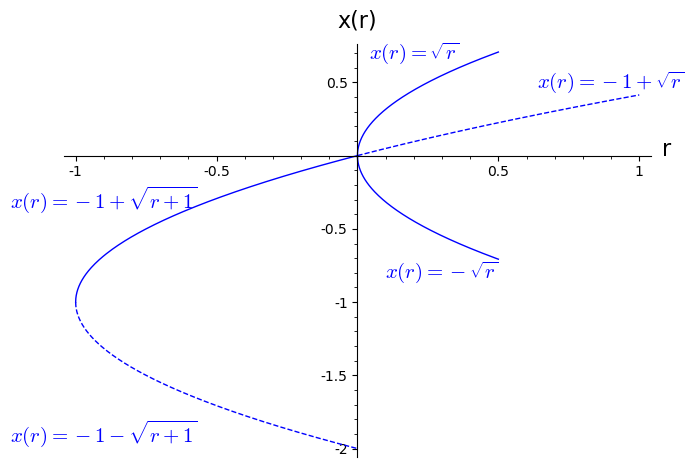
\includegraphics[height=4in]{/Users/ERICAGYEMANG/Desktop/Biomath/Figures/tmpsixxxx.jpg} 
        \caption[Figure 2.4: r>1]{The dashed curve in the graph represents unstability and the solid curve represents stability}
 \label{fig::model}
\end{figure}




\end{enumerate}





\cleardoublepage

\begin{thebibliography}{99}
\bibitem{r1} Linda Allen’s book, An Introduction to Mathematical Biology, Pearson, 2007


\end{thebibliography}

\end{document}